\documentclass[aspectratio=169]{beamer}
\usetheme{Madrid}
\usepackage[utf8]{inputenc}
\usepackage[T1]{fontenc}
\usepackage{tikz}
\usepackage{amssymb}
\usepackage{graphicx}
\setbeamertemplate{navigation symbols}{}
\setbeamercolor{title}{fg=white,bg=blue!65!cyan}
\setbeamercolor{frametitle}{fg=white,bg=blue!65!cyan}
\setbeamercolor{block title}{bg=blue!65!cyan!20,fg=black}
\setbeamercolor{block body}{bg=blue!65!cyan!8,fg=black}
\setbeamercolor{item}{fg=blue!65!cyan}
\setbeamercolor{itemize item}{fg=blue!65!cyan}
\setbeamertemplate{itemize item}[triangle]

\title{If/Else}
\subtitle{Decisions in real code — one comparison operator this week: ==}
\author{ByteForge --- Grade 8 --- App Builder}
\date{}

\begin{document}

\begin{frame}
    \titlepage
\end{frame}

\begin{frame}{Today's Plan}
    \begin{itemize}
        \item Odd or Even
        \item[$\bigstar$] BOSS --- Hot or Not
    \end{itemize}
\end{frame}

\begin{frame}{\texttt{\%} gives what's LEFT OVER after dividing}
    \large
    \begin{itemize}
        \item \texttt{number \% 2} is 0 for even numbers, 1 for odd
        \item The exact same MOD idea from Grade 7's blocks, now written as a real operator.
    \end{itemize}
\end{frame}


\begin{frame}{Real syntax: a colon, then indentation}
    \large
    \begin{itemize}
        \item \texttt{if number \% 2 == 0:} followed by an indented \texttt{print("Even")} is exactly what Grade 7's if/else BLOCKS actually compiled to underneath
        \item The visual nesting becomes real indentation.
    \end{itemize}
\end{frame}


\begin{frame}{BOSS — a different comparison, \texttt{>}}
    \large
    \begin{itemize}
        \item \texttt{if temperature > 25:}
        \item Swapping \texttt{==} for \texttt{>} handles a whole RANGE of values rather than one exact match, the same shape of decision applied to a genuinely different kind of question.
    \end{itemize}
\end{frame}

\begin{frame}{Real-World Examples}
    \large
    \begin{itemize}
        \item Every real app checking "is this number even" (splitting a bill, alternating row colors in a table) or "is this value above a threshold" (a thermostat, a speed-limit warning) runs exactly this if/else shape.
    \end{itemize}
\end{frame}


\begin{frame}{Image}
    \begin{center}
    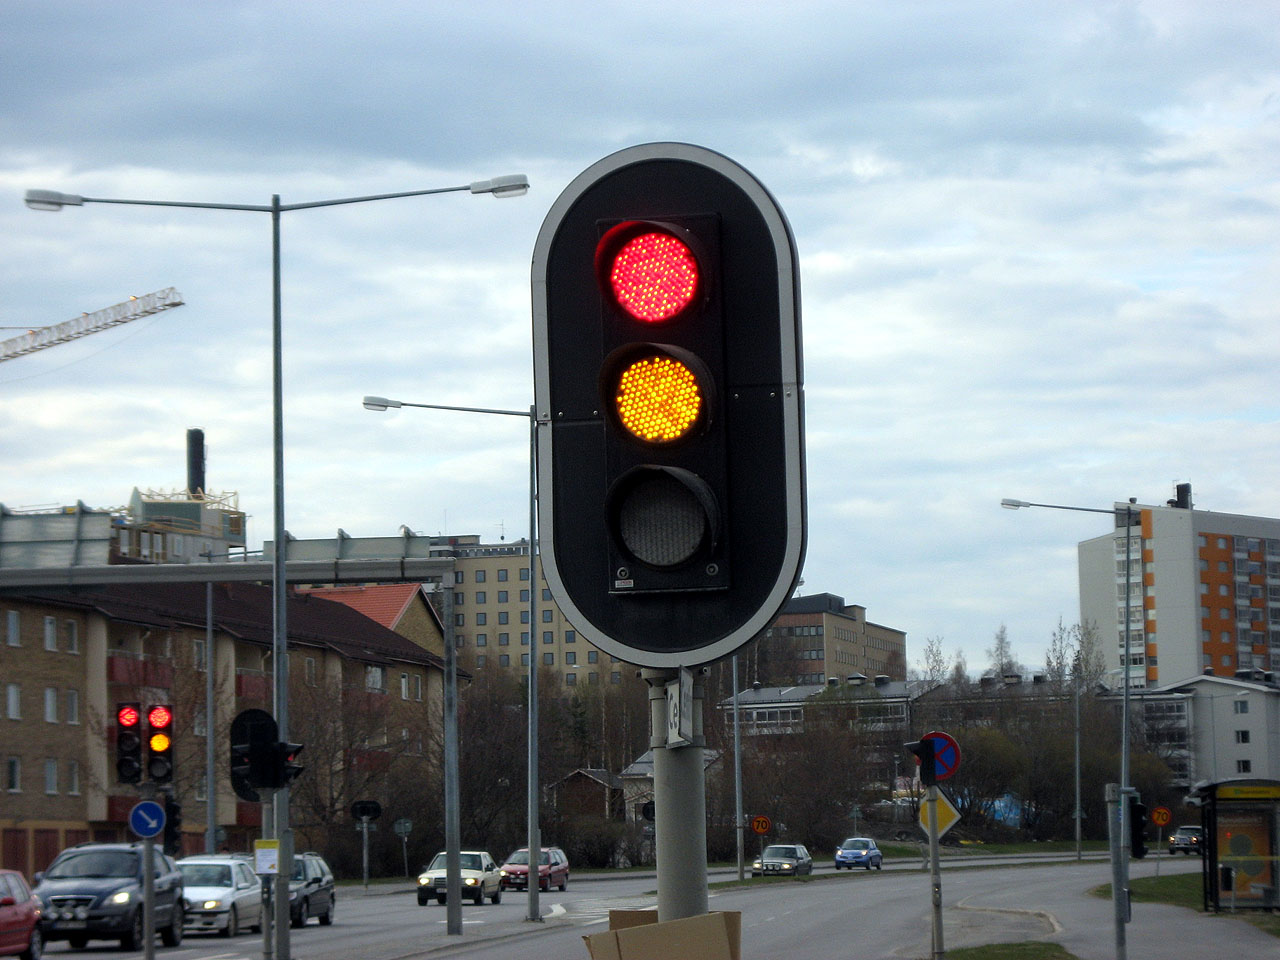
\includegraphics[width=0.5\textwidth]{images/traffic.jpg}

    \large A real branch, decided by a condition — the same if/else idea from this chapter.

    \small LED traffic lights, public domain (PD-self), via Wikimedia Commons
    \end{center}
\end{frame}

\begin{frame}{Let Them Discover}
    \Large
    Before typing anything: will \texttt{10 \% 2} be 0 or 1? Will \texttt{7 \% 2}? Write both guesses down, then check them against the actual rule this chapter teaches.
\end{frame}

\begin{frame}{Your Turn}
    \Large
    Open the student map, find \textbf{If/Else}, and work through it
    hands-on --- everything you just saw, they now do themselves.
\end{frame}

\end{document}
